\begin{frame}
    \frametitle{Kernel-Polynom-Methode (KPM)}
    \begin{itemize}
        \pause
        \item Polynomiale Annäherung der Spektraldichte
        \pause
        \item Leitet Koeffizienten aus der Momentenmethode ab
        \pause
        \item Zwei eng verwandte Varianten
        \pause
        \item Benutzt stochastische Sampling-Methode, die auf folgendem Resultat basiert:
    \end{itemize}
\end{frame}

\begin{frame}
    \frametitle{Theorem}
    \pause
    \begin{theorem}
        Sei $A = A^T \in \R^{n \times n}$ mit Spektralzerlegung $A = U \diag(\lambda_1, \dots, \lambda_n)U^T$ wobei $UU^T = \1_n$.\\
        Sei außerdem $\beta, v \in \R^n$ mit $v = U\beta$\\
        Gilt $v_i \sim \mathcal{N}(0, 1)$ i.i.d. für die Komponenten $\{v_i\}_{i = 1}^n$ von $v$, also $\E[v] = 0$ und $\E[vv^T] = \1_n$, dann
        $$\E[\beta \beta^T] = \1_n$$
    \end{theorem}
\end{frame}

\begin{frame}
    \frametitle{Beweisskizze}
    \pause
    \begin{proof}[Beweis Theorem 1]
        Es gilt
        $$\E[v] = \pause \E[U\beta] = \pause U\E[\beta] = \pause 0 \pause \implies \E[\beta] = 0$$
        \pause Weiterhin gilt, dass
        $$\E[vv^T] = \pause \E[(U\beta)(U\beta)^T] = \pause \E[U\beta \beta^TU^T] = \pause U \E[\beta \beta^T]U^T = \pause \1_n$$
        \pause Hieraus folgt, dass $\E[\beta \beta^T] = \1_n$
    \end{proof}
\end{frame}

\begin{frame}
    \frametitle{Resultat}
    \pause
    Sei $f(A)$ eine Matrixfunktion. Dann haben wir 
    \begin{align*}
        \E\left[v^Tf(A)v\right] & = \E\left[(U\beta)^Tf(U\Lambda U^T)(U\beta)\right]\\
         & = \E\left[\beta^TU^TUf(\Lambda)U^TU\beta\right]\\
         & = \E\left[\beta^Tf(\Lambda)\beta\right]\\
         & = \E\left[\sum_{j = 1}^n \beta_j^2 f(\lambda_j) \right]\\
         & = \sum_{j = 1}^n f(\lambda_j) \E\left[ \beta_j^2 \right]\\
         & = \sum_{j = 1}^n f(\lambda_j)
    \end{align*}
\end{frame}

\begin{frame}
    \frametitle{Tschebyschev-Polynome}
    Mit Hilfe der trigonometrischen Funktionen können die Tschebyschev wie folgt ausgedrückt werden:
    \[ T_k(t) =
    \begin{cases}
        \cos(k \arccos(t))            & \quad \text{für } k \in [-1, 1]\\
        \cosh(k \arcosh(t))           & \quad \text{für } k > 1\\
        (-1)^k \cosh(k \arcosh(-t))   & \quad \text{für } k < -1
    \end{cases}
    \]
    \pause
    Es gilt außerdem die Rekursionsformel
    $$T_{k + 1}(t) = 2tT_k(t) - T_{k - 1}(t)$$
\end{frame}

\begin{frame}
    \frametitle{Transformation der Eigenwerte}
    \pause
    Wir benutzen im Folgenden $T_k(t) = \cos(k \arccos(t))$ um die Dirac-Dichte zu erweitern.\\
    \pause
    Wir müssen uns daher auf Matrizen beschränken, deren Eigenwerte im Intervall $[-1, 1]$ liegen.\\
    \pause
    Seien daher $\lambda_{us}$ und $\lambda_{os}$ jeweils die untere bzw. obere Schranke für die Eigenwerte von $A$.
    Definiere
    $$c := \frac{\lambda_{us} + \lambda_{os}}{2} \quad \text{und} \quad d := \frac{\lambda_{os} - \lambda_{us}}{2}$$
    Dann ist $B = \frac{A - c*\1_n}{d}$ eine Matrix mit Eigenwerten im Intervall $[-1, 1]$
\end{frame}

\begin{frame}
    \frametitle{Erweiterung der Delta-Distribution}
    Berechne zunächst
    $$\hat{\phi}(t) = \sqrt{1 - t^2} \phi(t) = \sqrt{1 - t^2} \times \frac{1}{n} \sum_{j = 1}^n \delta(t - \lambda_j)$$
    Nun erweitern wir
    $$\hat{\phi}(t) = \sum_{k = 0}^{\infty} \mu_k T_k(t)$$
    im Sinne von
    $$\int \limits_{-1}^1 \hat{\phi}(t) g(t) \dt = \int \limits_{-1}^1 \sum_{k = 0}^{\infty} \mu_k T_k(t) g(t) \dt$$
    für $g \in \SR$
\end{frame}

\begin{frame}
    \frametitle{Momentenmethode}
    \begin{align*}
        \mu_k &= \frac{2 - \delta_{k0}}{\pi} \int\limits_{-1}^1 \frac{1}{\sqrt{1 - t^2}} T_k(t) \hat\phi(t) \dt\\
        &= \frac{2 - \delta_{k0}}{\pi} \int\limits_{-1}^1 \frac{1}{\sqrt{1 - t^2}} T_k(t) \sqrt{1 - t^2} \phi(t) \dt\\
        &= \frac{2 - \delta_{k0}}{n \pi} \sum_{j = 1}^n T_k(\lambda_j)\\
        &= \frac{2 - \delta_{k0}}{n \pi} \Spur(T_k(A))
    \end{align*}
\end{frame}

\begin{frame}
    \frametitle{Weitere Parameter}
    Es folgt, dass
    $$\zeta_k = \frac{1}{n_{vec}} \sum_{l = 1}^{n_{vec}} \left( v_0^{(l)} \right)^T T_k(A) v_0^{(l)}$$
    ein guter Schätzer für $\Spur(T_k(A))$ ist und damit
    $$\mu_k \approx \frac{2 - \delta_{k0}}{n \pi} \zeta_k$$
\end{frame}

\begin{frame}
    \frametitle{Berechnung der $\zeta_k$}
    Sei im Folgenden $v_0 \equiv v_0^{(l)}$
    Berechne nun
    $$T_{k + 1}(A)v_0 = 2 A T_k(A) v_0 - T_{k - 1}(A) v_0$$
    Für $v_k \equiv T_k(A)v_0$ gilt also, dass
    $$v_{k + 1} = 2 A v_k - v_{k - 1}$$
\end{frame}

\begin{frame}
    \frametitle{Definition $\tilde{\phi}_M(t)$}
    Sobald die $\{ \mu_k \}$ bestimmt sind, wäre die Erweiterung theoretisch durch
    $$\phi(t) = \frac{1}{\sqrt{1 - t^2}} \hat{\phi}(t)$$
    gegeben. Allerdings gilt
    $$\lim \limits_{k \to \infty} \mu_k \to 0$$
    und wir interessieren uns nur für $T_k(t)$ mit $k \leq M$\\
    Daher schätzen wir $\phi$ durch
    $$\tilde{\phi}_M(t) = \frac{1}{\sqrt{1 - t^2}} \sum_{k = 0}^{M} \mu_k T_k(t)$$
\end{frame}

\begin{frame}
    \frametitle{Der Pseudocode}
    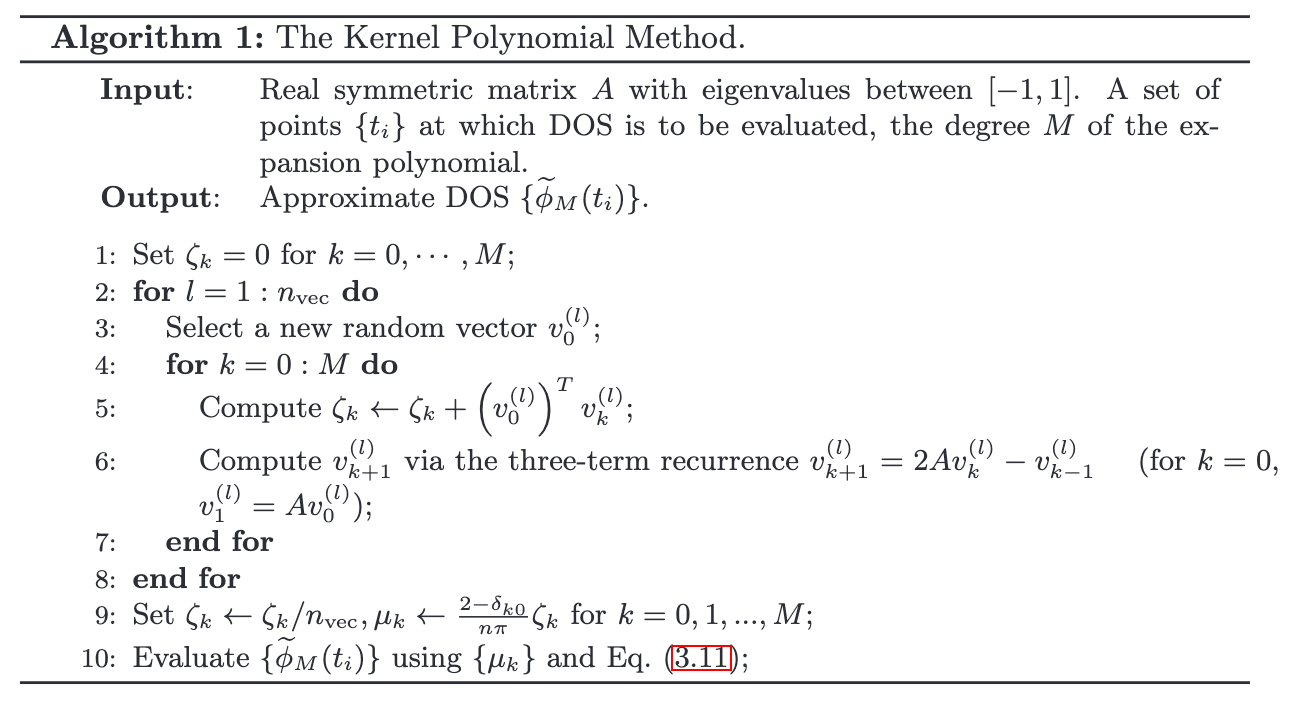
\includegraphics[height = 6.15cm]{./Bilder/Pseudocode.png}
\end{frame}